%%%%%%%%%%%%%%%%%%%%%%%%%%%%% Define Article %%%%%%%%%%%%%%%%%%%%%%%%%%%%%%%%%%
\documentclass{article}
%%%%%%%%%%%%%%%%%%%%%%%%%%%%%%%%%%%%%%%%%%%%%%%%%%%%%%%%%%%%%%%%%%%%%%%%%%%%%%%

%%%%%%%%%%%%%%%%%%%%%%%%%%%%% Using Packages %%%%%%%%%%%%%%%%%%%%%%%%%%%%%%%%%%
\usepackage{geometry}
\usepackage{graphicx}
\usepackage{amssymb}
\usepackage{amsmath}
\usepackage{amsthm}
\usepackage{empheq}
\usepackage{mdframed}
\usepackage{booktabs}
\usepackage{lipsum}
\usepackage{graphicx}
\usepackage{color}
\usepackage{psfrag}
\usepackage{pgfplots}
\usepackage{bm}
\usepackage{biblatex}
\usepackage{hyperref}
\usepackage{listings}
\usepackage{pythonhighlight}
%%%%%%%%%%%%%%%%%%%%%%%%%%%%%%%%%%%%%%%%%%%%%%%%%%%%%%%%%%%%%%%%%%%%%%%%%%%%%%%

% Other Settings

\addbibresource{references.bib}
\graphicspath{ {./assets/} }

%%%%%%%%%%%%%%%%%%%%%%%%%% Page Setting %%%%%%%%%%%%%%%%%%%%%%%%%%%%%%%%%%%%%%%
\geometry{a4paper}

%%%%%%%%%%%%%%%%%%%%%%%%%% Define some useful colors %%%%%%%%%%%%%%%%%%%%%%%%%%
\definecolor{ocre}{RGB}{243,102,25}
\definecolor{mygray}{RGB}{243,243,244}
\definecolor{deepGreen}{RGB}{26,111,0}
\definecolor{shallowGreen}{RGB}{235,255,255}
\definecolor{deepBlue}{RGB}{61,124,222}
\definecolor{shallowBlue}{RGB}{235,249,255}
%%%%%%%%%%%%%%%%%%%%%%%%%%%%%%%%%%%%%%%%%%%%%%%%%%%%%%%%%%%%%%%%%%%%%%%%%%%%%%%

%%%%%%%%%%%%%%%%%%%%%%%%%% Define an orangebox command %%%%%%%%%%%%%%%%%%%%%%%%
\newcommand\orangebox[1]{\fcolorbox{ocre}{mygray}{\hspace{1em}#1\hspace{1em}}}
%%%%%%%%%%%%%%%%%%%%%%%%%%%%%%%%%%%%%%%%%%%%%%%%%%%%%%%%%%%%%%%%%%%%%%%%%%%%%%%

%%%%%%%%%%%%%%%%%%%%%%%%%%%% English Environments %%%%%%%%%%%%%%%%%%%%%%%%%%%%%
\newtheoremstyle{mytheoremstyle}{3pt}{3pt}{\normalfont}{0cm}{\rmfamily\bfseries}{}{1em}{{\color{black}\thmname{#1}~\thmnumber{#2}}\thmnote{\,--\,#3}}
\newtheoremstyle{myproblemstyle}{3pt}{3pt}{\normalfont}{0cm}{\rmfamily\bfseries}{}{1em}{{\color{black}\thmname{#1}~\thmnumber{#2}}\thmnote{\,--\,#3}}
\theoremstyle{mytheoremstyle}
\newmdtheoremenv[linewidth=1pt,backgroundcolor=shallowGreen,linecolor=deepGreen,leftmargin=0pt,innerleftmargin=20pt,innerrightmargin=20pt,]{theorem}{Theorem}[section]
\theoremstyle{mytheoremstyle}
\newmdtheoremenv[linewidth=1pt,backgroundcolor=shallowBlue,linecolor=deepBlue,leftmargin=0pt,innerleftmargin=20pt,innerrightmargin=20pt,]{definition}{Definition}[section]
\theoremstyle{myproblemstyle}
\newmdtheoremenv[linecolor=black,leftmargin=0pt,innerleftmargin=10pt,innerrightmargin=10pt,]{problem}{Problem}[section]
%%%%%%%%%%%%%%%%%%%%%%%%%%%%%%%%%%%%%%%%%%%%%%%%%%%%%%%%%%%%%%%%%%%%%%%%%%%%%%%

%%%%%%%%%%%%%%%%%%%%%%%%%%%%%%% Plotting Settings %%%%%%%%%%%%%%%%%%%%%%%%%%%%%
\usepgfplotslibrary{colorbrewer}
\pgfplotsset{width=8cm,compat=1.9}
%%%%%%%%%%%%%%%%%%%%%%%%%%%%%%%%%%%%%%%%%%%%%%%%%%%%%%%%%%%%%%%%%%%%%%%%%%%%%%%

%%%%%%%%%%%%%%%%%%%%%%%%%%%%%%% Title & Author %%%%%%%%%%%%%%%%%%%%%%%%%%%%%%%%
\title{Reverse Engineering Proprietary Bluetooth Protocol}
\author{Yuva Shankar Y, Rammohan M, Puneeth, Haarish Ahmed, Pranaov S}
\date{November 18, 2024}
%%%%%%%%%%%%%%%%%%%%%%%%%%%%%%%%%%%%%%%%%%%%%%%%%%%%%%%%%%%%%%%%%%%%%%%%%%%%%%%


\begin{document}

\maketitle
\tableofcontents
\newpage


\section{Introduction}

Bluetooth protocol is a short range wireless communication protocol.
It is a very short range communication protocol.
It is primarily used in intercommunication of mobile devices.

The Bluetooth Special Interest Group (SIG)\cite{bt-sig}~\cite{bt-about} was formed and announced on May 20, 1998.
It was established by Ericsson, IBM, Intel, Nokia and Toshiba, and later joined by many other companies


\section{Protocols}

The data exchange in Bluetooth uses a variety of different protocols.
Core Protocols are defined by SIG~\cite{bt-about}\cite{bt-sig}.

It is split into two parts briefly, the ``controller stack'' and ``host stack''.
The controller stack is implemented in on the low level device (mostly the chip), and the host stack is a part of the operating system, or the software that connects to the host stack.

\subsection{Controller stack}

There are 5 layers in the controller stack, namely:

\begin{enumerate}
  \item Asynchronous Connection-Less (ACL)
  \item Synchrous Connection-Oriented Link (SCO)
  \item Link Management Protocol (LMP)
  \item Host Controller Interface (HCI)
  \item Low Energy Link Layer (LE LL)
\end{enumerate}

\subsection{Host Stack}

The topic of interest of this report uses the Host stack.

The components of the Host stack are:

\begin{enumerate}
  \item Logical link control and adaptation protocol (L2CAP):

    L2CAP is used to pass packets either to HCI, or directly to the ACL Link
    Its functions include:

    \begin{itemize}
      \item Multiplexing data between different higher layer protocol 
      \item Segmentation and reassembly of packets
      \item One way communication
    \end{itemize}

  \item Radio frequency communication (RFCOMM):

    RFCOMM is made on top of L2CAP protocol, providing emulated RS-232 serial ports~\cite{bt-specs}\cite{bt-arch}.

    It provides simple reliable data stream to user, similar to TCP.\@

  \item Service discovery protocol (SDP):

    It is used to allow devices to discover what servcies weach device support, and what parameters are needed to connect to them.
    Each service is identified with a UUID, with official services assigned short form UUID (16 instead of 128 bits)

  \item Telephony control protocol (TCP):

    Used to setup and control speech and data calls between Bluetooth devices.

  \item Audio/video control transport protocol (AVCTP):

    Used to transfer AV/C commands over an L2CAP channel. Example: Music control buttons.

  \item Audio/video data transport protocol (AVDTP):

    Stream music to stereo headsets over an L2CAP channel.

  \item Object exchange (OBEX):

    Facilitates exchange of binary objects between devices. Example: used to transfer files from a device to a printer.

  \item Low Energy Attribute Protocol (ATT):

    Similar to SDP but adapted for Low Energy Bluetooth (Bluetooth LE). Bound to L2CAP.\@

  \item Low energy security manager protocol (SMP):

    Use for pairing and transport of keys in Bluetooth LE implementations. Bound to L2CAP.\@
\end{enumerate}

\section{Reverse-engineering the proprietary protocol}

There exists well-documented protocols like the ACTCP to control music playback,
or the TCP to setup and allow bluetooth calls.

But there are also exists RFCOMM protocol to send arbitrary commands emulating serial ports.
It is often used for arbitrary data communications which cannot be covered in the standard protocols,
like health data from smart watches, proprietary headphone control apps, bluetooth enabled weighing scales, etc.

The process of reverse-engineering RFCOMM protocols typically involves dumping packtes and analyzing them,
or trying to find how the packets are sent from the source (de-compilation of the app)\cite{bt-re-article}.

In this case, we will be reverse-engineering the proprietary stack of a bluetooth headphone Soundcore Q20i which is used to control ANC and sound profiles.

\section{Dumping the packets}

The Soundcore Q20i headphones use a proprietary app called Soundcore (\href{https://play.google.com/store/apps/details?id=com.oceanwing.soundcore}{Google Play Store}),
to manage ANC settings, equalizer settings and various other settings of the headphones.
\begin{center}
  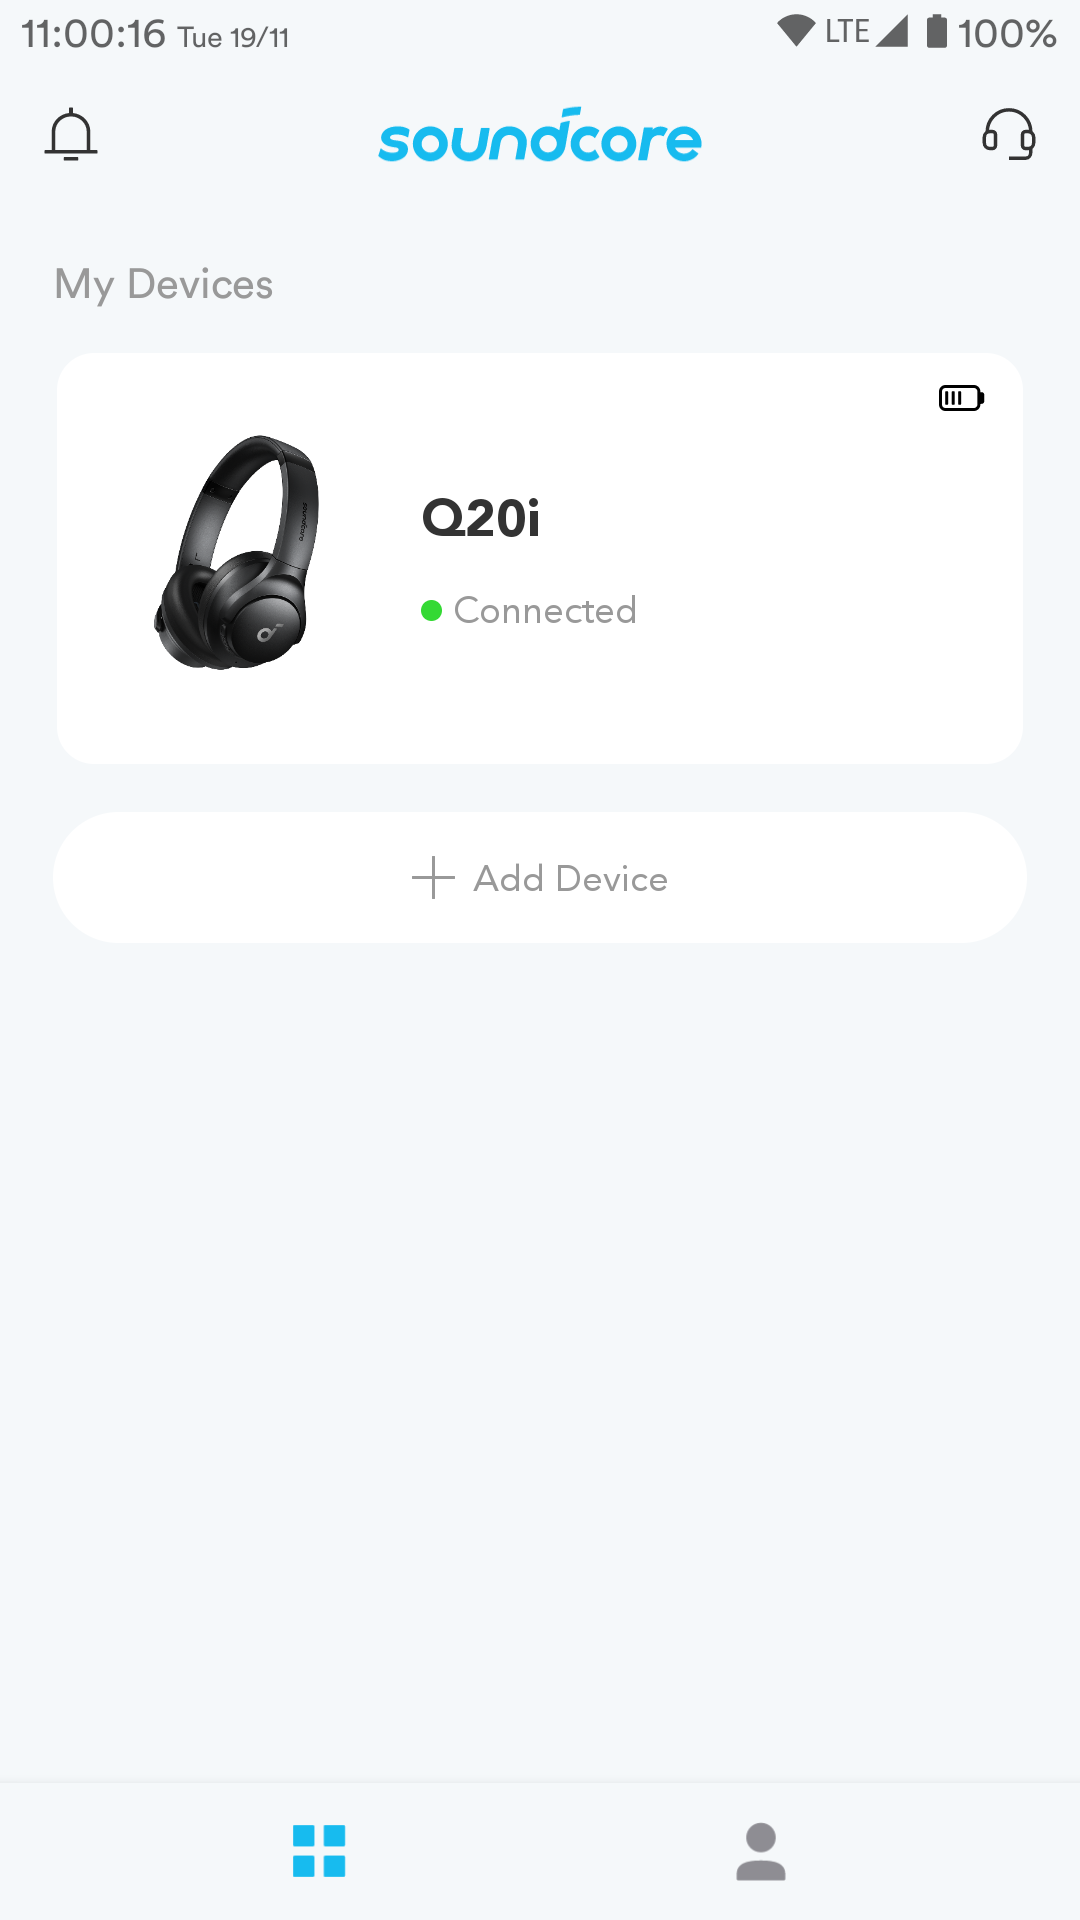
\includegraphics[width=150px]{soundcore-app-connected}
  ~
  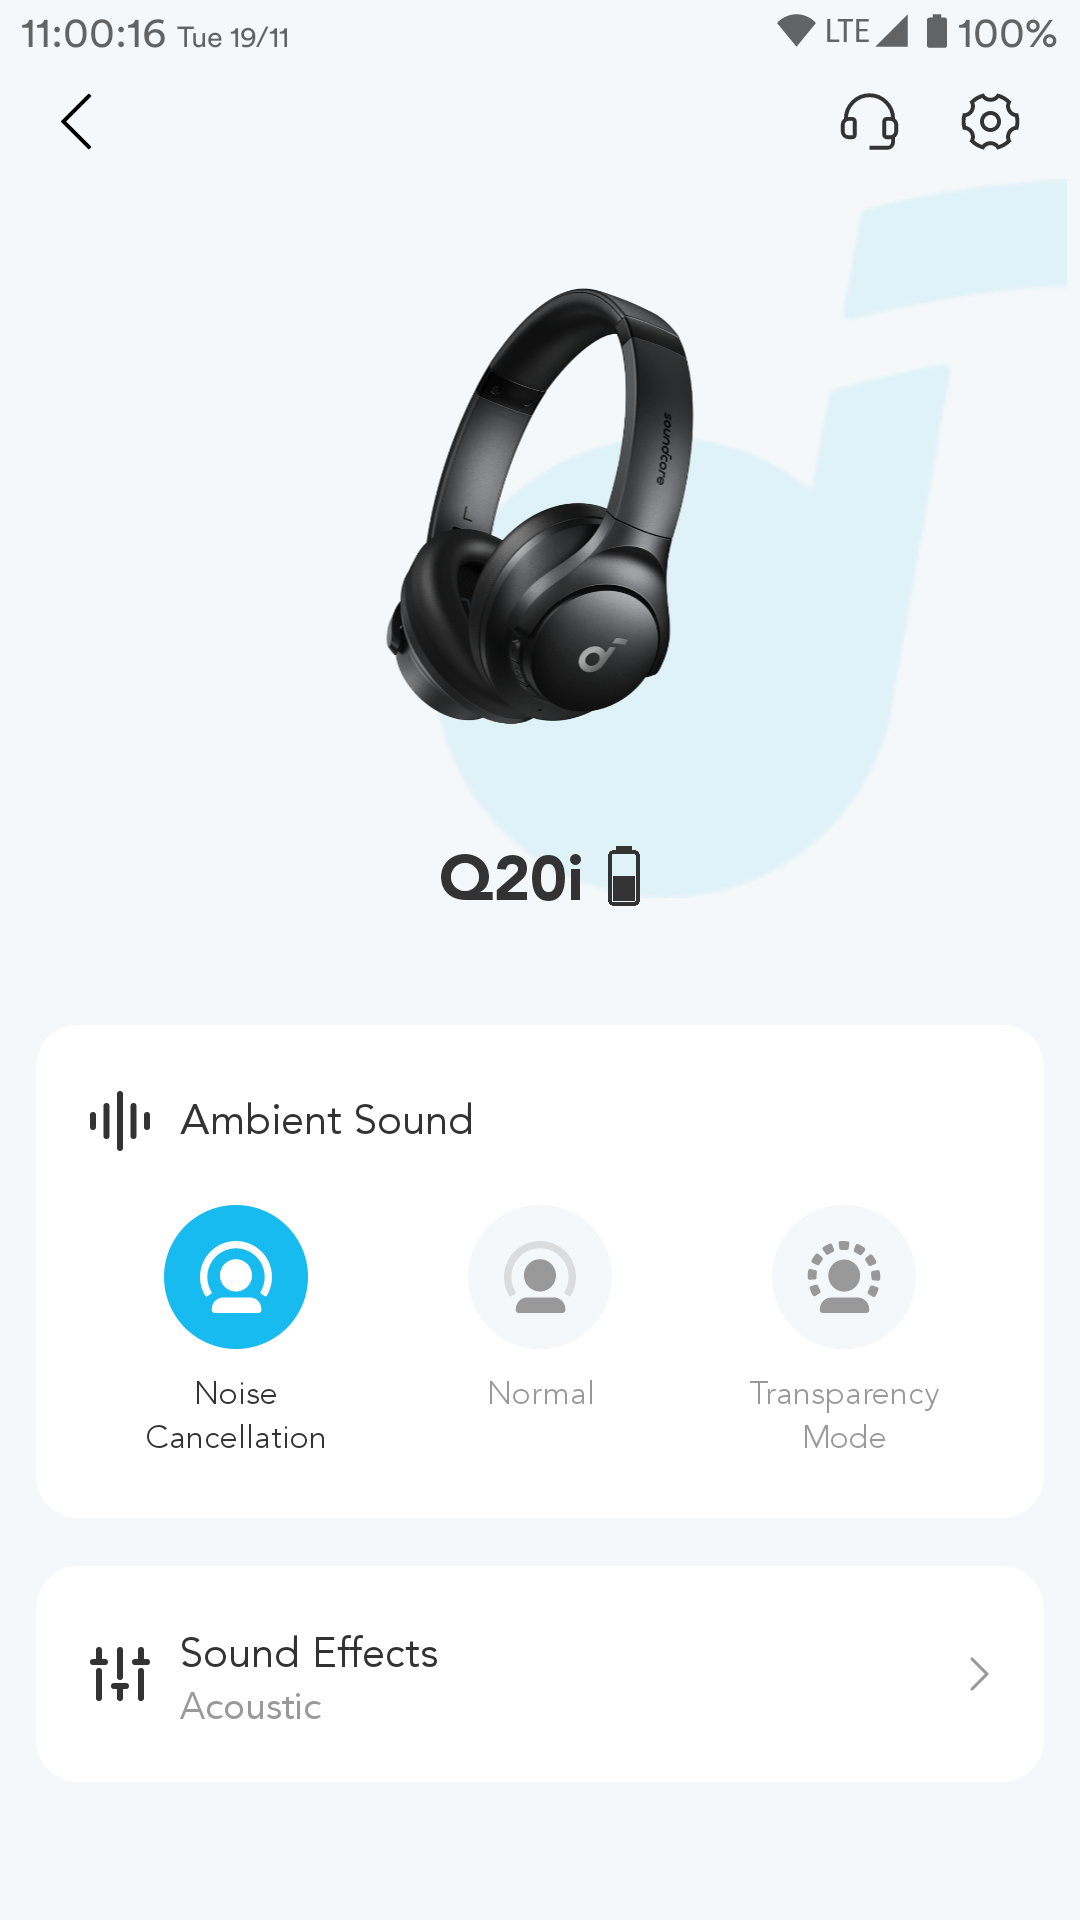
\includegraphics[width=150px]{soundcore-app-device}
\end{center}

The approach taken is to dump the bluetooth packets and analyzing them, instead of app-decompilation.

The Android operating system provides an option to snoop (and dump) all the bluetooth packets sent from the device.
This feature is called the HCI Snoop Log. Usually, it is present under developer settings.
After enabling the HCI snoop logging, we can now snoop all packet data through the bluetooth interface.

After performing some actions on the app (example, setting to ANC, then Transparency mode, etc),
Bluetooth is turned off to stop HCI packet dumping,
and the file is copied over to a system with packet visualizing/analyzing software like Wireshark.
The file is normally located in \texttt{/sdcard/btsnoop\_hci.log} or \texttt{/data/misc/bluetooth/logs/btsnoop\_hci.log}


\section{Packet analysis}

The HCI snoop log \texttt{btsnoop\_hci.log} is opened using Wireshark for packet analysis.
\begin{center}
  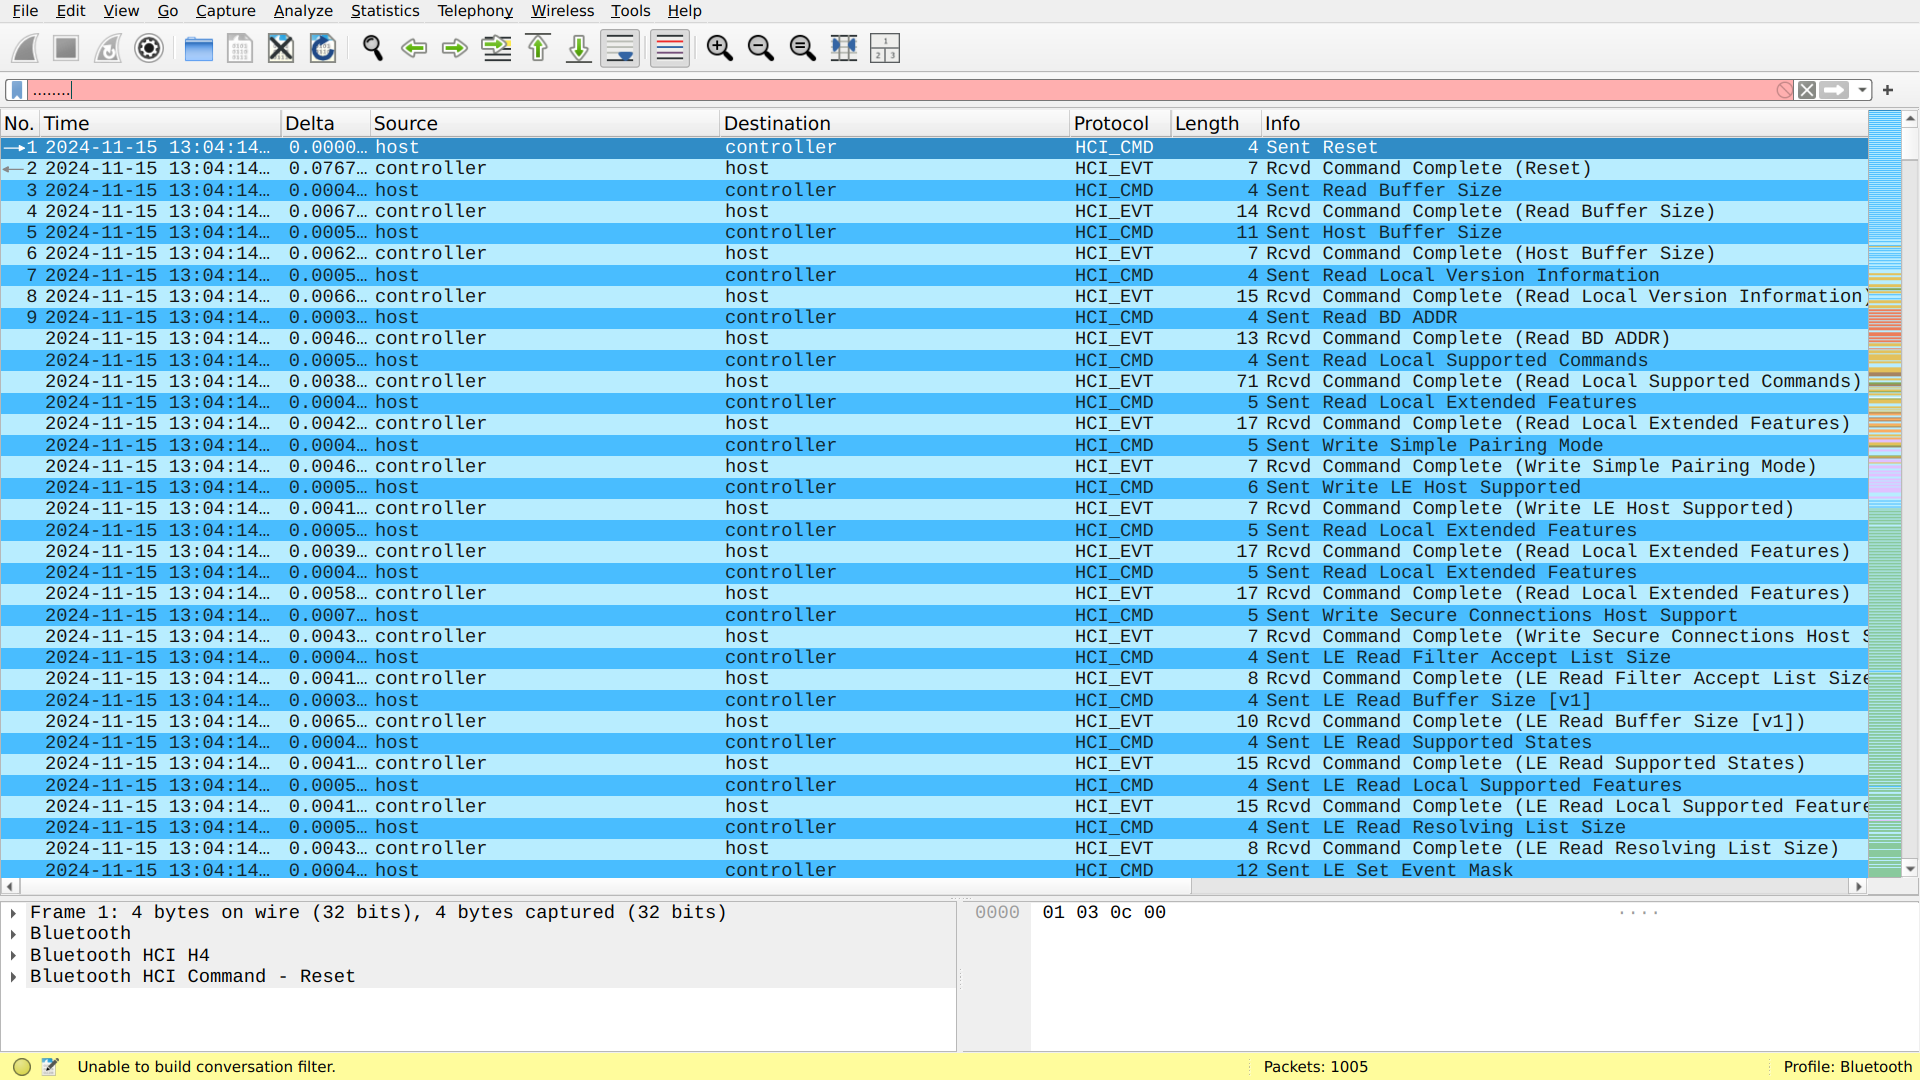
\includegraphics[width=400px]{wireshark-launch}
\end{center}

Packets going to and from our host device (Android device) and the controller can be observed.

By sorting the packets according to their destination and navigating to packets with destination Soundcore Q20i,
the packet analysis can be made easier.
\begin{center}
  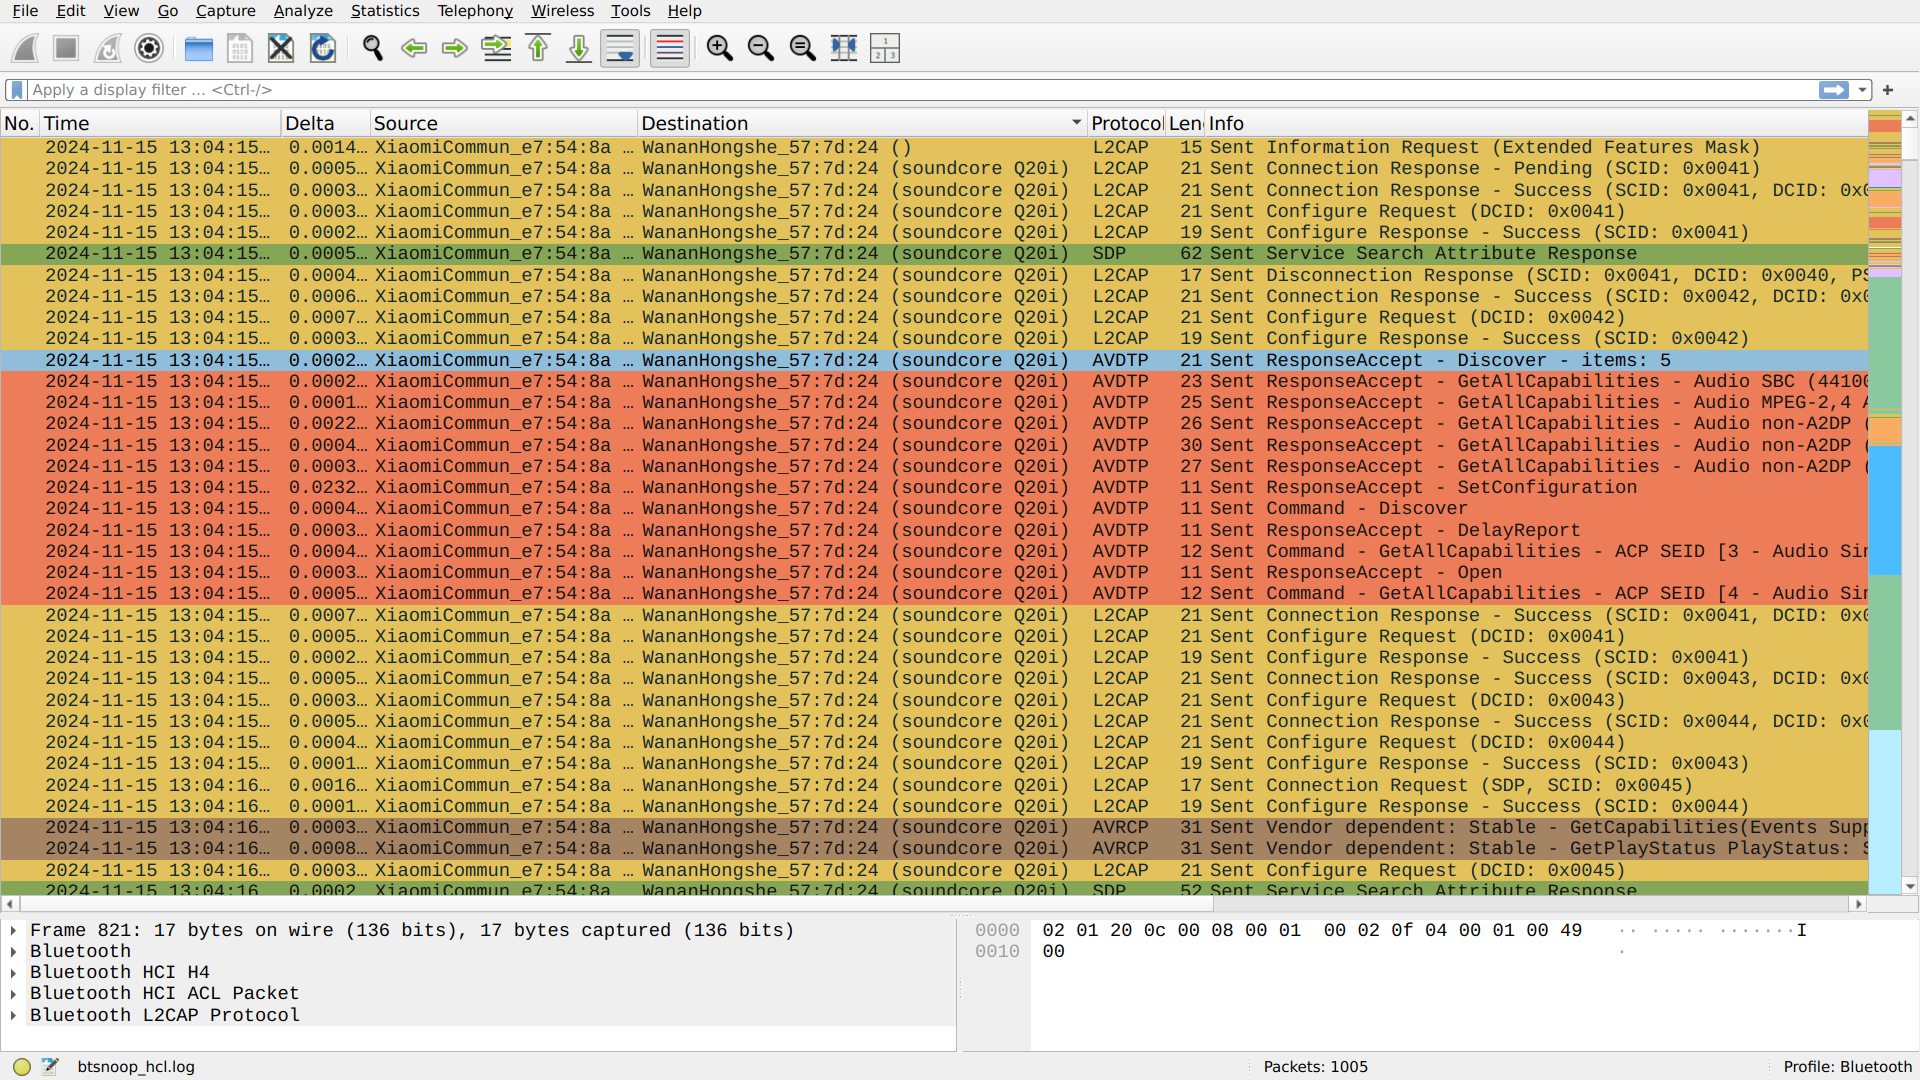
\includegraphics[width=400px]{wireshark-sorted}
\end{center}

In this case, there are an SDP packet originating from the Android device to Soundcore Q20i headphones to discover the capabilities of the device.
There are a few AVDTP packets. They take place over the L2CAP channel.

\newpage

By scrolling down to find the packets sent by the Soundcore App (while changing noise cancelling mode),
we find a few RFCOMM packets. The modes were switched with an interval of 10 seconds and times were noted.
\begin{center}
  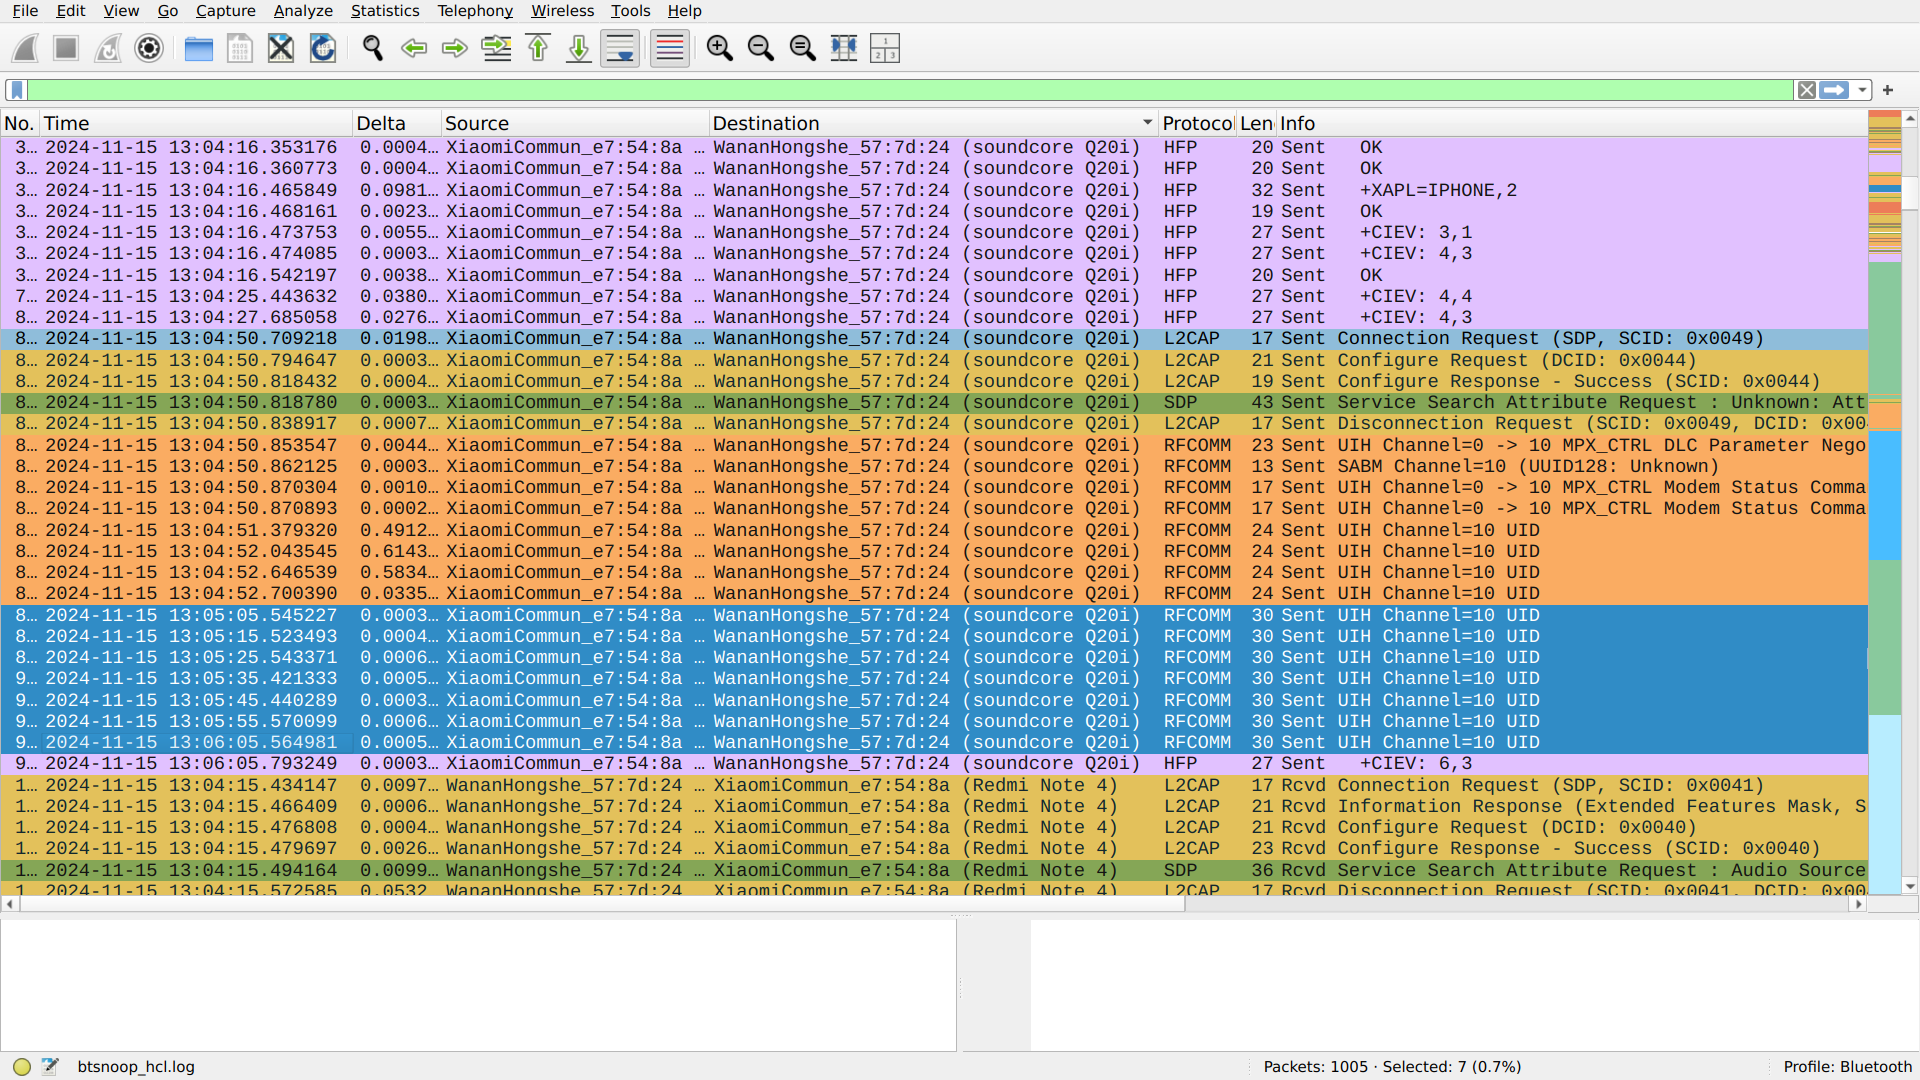
\includegraphics[width=400px]{wireshark-rfcomm}
\end{center}

There exists 7 RFCOMM packets sent with an interval of 10 seconds each, which correlates perfectly with the actions done on the mobile app.

With this, it can be concluded that these are the packets responsible for changing the noise-cancelling mode on the headphones.

\newpage

Viewing one RFCOMM packet in detail, the following can be observed:
\begin{center}
  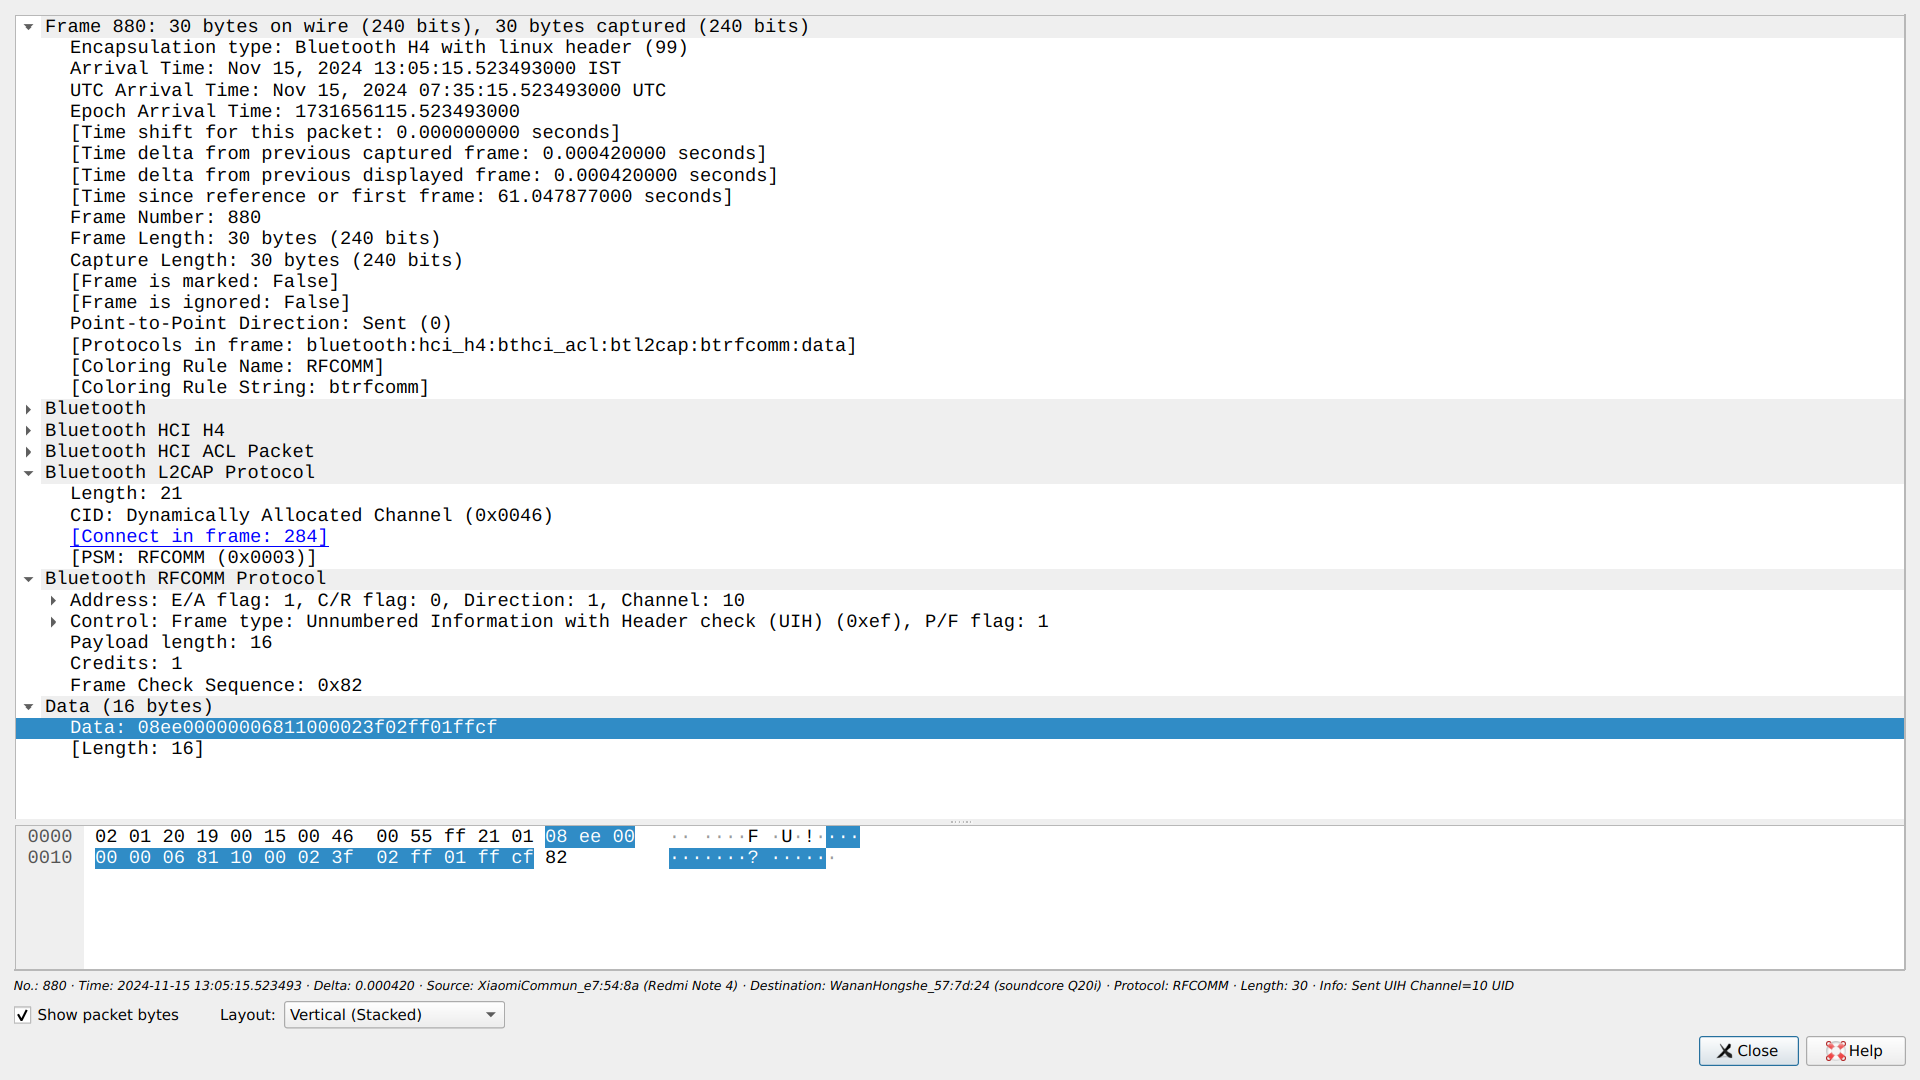
\includegraphics[width=400px]{wireshark-detailed-packet}
\end{center}

\begin{enumerate}
  \item It is an RFCOMM protocol packet 
  \item It is over the L2CAP protocol 
  \item There are a total of 30 bytes 
  \item The RFCOMM packet as 16 bytes of data: \texttt{08ee00000006811000023f02ff01ffcf}
  \item It is a hex string
\end{enumerate}

By comparing it to the timings chart, this data corresponds to setting the noise-cancelling mode to normal mode.
\\\\
Similarly, the packet data for ANC mode is \texttt{08ee00000006811000003f02ff01ffcd} and that for Transparency mode is \texttt{08ee00000006811000013f02ff01ffce}.
\\\\
To conclude, it is required to send this 16 bytes of data over RFCOMM protocol to the headphone to change the noise-cancelling mode.

\section{Reimplementation in code}

Python is used for this application since it is easy to write and debug,
and has a huge 3rd-party support to prevent reinventing the wheel.
\\
The socket\cite{py-socket} library of python allows access to the low-level networking interface.
It is platform dependent since it needs to make calls to the OS's APIs.
\\\\
It is required to send the 16 bytes of RFCOMM packet to the device.

\subsection{Python implementation}

Firstly, the socket library is imported and a new socket object is created with \texttt{BTPROTO.RFCOMM} protocol.

\begin{python}
import socket
sock = socket.socket(
    socket.AF_BLUETOOTH, socket.SOCK_STREAM, socket.BTPROTO_RFCOMM
)
\end{python}

Then we create a function to simplify sending the hex data to the device

\begin{python}
from time import sleep

def send(data):

    # print(data)
    sock.send(bytearray.fromhex(data))
    sleep(0.1)
\end{python}

Since RFCOMM can listen on any port, we can use a \pyth{for} loop to check the ports from 1 to 30\cite{rfcomm-port}
A new socket instance is created for each port and tries to connect using RFCOMM protocol. And the function returns if connection is successful (after closing the socket)
\begin{python}
from time import sleep

def getPort(macaddress):
    print(macaddress)
    for x in range(1, 31):
        try:
            s = socket.socket(
                socket.AF_BLUETOOTH, socket.SOCK_STREAM, socket.BTPROTO_RFCOMM
            )
            s.connect((macaddress, x))
            sleep(0.1)
            s.close()
            return x
        except OSError:
            pass
  return None
\end{python}

Finally, the packet data can be sent to the headphones\cite{soundcore-ref}.
\begin{python}
def main():
  macaddress = "B0:38:E2:XX:XX:XX"
  port = getPort(macaddress)
  sock.connect((macaddress, port))

  normal: str = "08ee00000006811000023f02ff01ffcf"
  anc: str = "08ee00000006811000003f02ff01ffcd"
  transparency: str = "08ee00000006811000013f02ff01ffce"

  send(anc)
  sleep(0.5)
  send(normal)
  sleep(0.5)
  send(transparency)
  sleep(0.5)

if __name__ in "__main__"::
  main()
\end{python}

\section{Conclusion}

Bluetooth reverse-engineering can be made easy thanks to the arsenal of tools present.

A reimplementation of the mobile app is currently in works, which can be viewed at \href{https://github.com/pranaovs/Soundcore-API}{https://github.com/pranaovs/Soundcore-API}.

\printbibliography

\end{document}
